% Session set-up and alignment between a host and a guest headset (NetworkSession.cs, SharedSpace.cs).
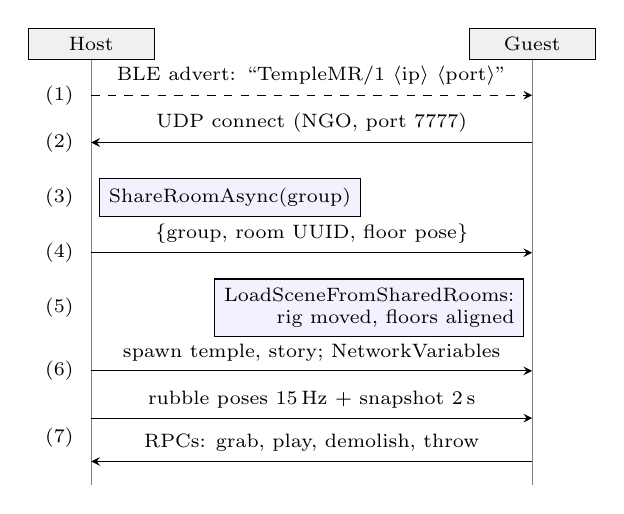
\begin{tikzpicture}[
  font=\scriptsize,
  msg/.style={->, >=stealth},
  note/.style={align=left, font=\scriptsize},
]
\def\top{0}
\def\bot{-5.6}
\node[draw, fill=gray!12, minimum width=1.6cm] (H) at (0,\top) {Host};
\node[draw, fill=gray!12, minimum width=1.6cm] (G) at (5.6,\top) {Guest};
\draw[gray] (H.south) -- (0,\bot);
\draw[gray] (G.south) -- (5.6,\bot);

\draw[msg, dashed] (0,-0.65) -- node[above, note] {BLE advert: ``TempleMR/1 $\langle$ip$\rangle$ $\langle$port$\rangle$''} (5.6,-0.65);
\node[note, anchor=east] at (-0.1,-0.65) {(1)};
\draw[msg] (5.6,-1.25) -- node[above, note] {UDP connect (NGO, port 7777)} (0,-1.25);
\node[note, anchor=east] at (-0.1,-1.25) {(2)};
\node[note, anchor=east, align=right] at (-0.1,-1.95) {(3)};
\node[note, anchor=west, draw, fill=blue!5] at (0.1,-1.95) {ShareRoomAsync(group)};
\draw[msg] (0,-2.65) -- node[above, note] {\{group, room UUID, floor pose\}} (5.6,-2.65);
\node[note, anchor=east] at (-0.1,-2.65) {(4)};
\node[note, anchor=east, draw, fill=blue!5, align=right] at (5.5,-3.35) {LoadSceneFromSharedRooms:\\rig moved, floors aligned};
\node[note, anchor=east] at (-0.1,-3.35) {(5)};
\draw[msg] (0,-4.15) -- node[above, note] {spawn temple, story; NetworkVariables} (5.6,-4.15);
\node[note, anchor=east] at (-0.1,-4.15) {(6)};
\draw[msg] (0,-4.75) -- node[above, note] {rubble poses 15\,Hz + snapshot 2\,s} (5.6,-4.75);
\draw[msg] (5.6,-5.3) -- node[above, note] {RPCs: grab, play, demolish, throw} (0,-5.3);
\node[note, anchor=east] at (-0.1,-5.0) {(7)};
\end{tikzpicture}
